% To-Dos:

\chapter{Thinking outside the box: A vision of ambient learning displays} % Write in your own chapter title

%\begin{quote}
%\textbf{Abstract:} With a focus on the situated support of informal and non-formal
%learning scenarios in ubiquitous learning environments, the presented paper outlines the authors� vision of ambient learning displays � enabling
%learners to view, access, and interact with contextualised digital content
%presented in an ambient way. The vision is based on a detailed exploration of
%the characteristics of ubiquitous learning and a deduction of informational,
%interactional, and instructional aspects to focus on. Towards the vision essential
%research questions and objectives as well as a conceptual framework that
%acquires, channels, and delivers the information framed in the learning process
%are presented. To deliver scientific insights into the authentic learning support
%in informal and non-formal learning situations and to provide suggestions for
%the future design of ambient systems for learning the presented paper concludes with a
%research agenda proposing a research project including a discussion of related
%issues and challenges.
%\end{quote}
\vfill
The first part of the thesis looks into the theoretical foundations for the following research. This chapter starts with outlining the vision of ambient learning displays and elaborating on a conceptual framework. Relevant research findings, models, design dimensions, and taxonomies are examined to deduce informational, interactional, and instructional aspects to focus on. The resulting conceptual framework consists of parts dedicated to user and context data acquisition, channelling of information, and delivery of contextualised information framed in a learning process. The chapter concludes with a research agenda.
\vspace{3em}

This chapter is published as: B�rner, D., Kalz, M., and Specht, M. (2011). Thinking outside the box � A vision on ambient learning displays. \textit{International Journal of Technology Enhanced Learning}, 3(6), 627�642.
\clearpage

\section{Introduction and background}

Within the knowledge society the constant update of knowledge and competences of
individuals is becoming a necessity to solve some urgent problems of the 21st century.
From a lifelong learning perspective users should be enabled to participate in training and
learning activities throughout their lifetime, be it within formal educational programs or
non-formal respectively informal educational activities \citep{Smith2009}. We differentiate
between educational activities conducted in the context of an educational institution
(formal learning) and activities, which are planned and conducted outside of educational
institutions and curriculums (non-formal) or even activities which are unplanned or
accidental (informal learning). At the same time the technical prospects are changing.
The amount of mobile consumer devices is rapidly growing and predicted to be ten times
higher than the amount of stationary devices \citep{MorganStan2009}. Notably the used
technology becomes also embedded into the physical environment providing a new
digital layer that supplements existing facilities and architectures, ranging from
automobiles, over living rooms, up to buildings that become smart. Furthermore, the
mobile internet is adopted much faster than the traditional desktop internet. In a rather
short period of time after launching respective mobile services attracted already more
users than desktop services did in a comparable period and the mobile data traffic is
increasing continuously \citep{MorganStan2009}.

This growing adoption of mobile technologies accompanied with ubiquitous
connectivity as well as the increasing pervasiveness of information technology are
changing the conditions for lifelong learning. Especially informal learning is becoming
more and more prominent in mobile learning approaches \citep{Ally2009b}. While rethinking
the relationship of environment, technology, and learning, the promises of mobile and
ubiquitous learning need to be explored to build a bridge between different contexts and
situations learners are operating in. This is strongly related to authentic learning theories
and situated learning. Authentic learning �allows students to explore, discover, discuss,
and meaningfully construct concepts and relationships in contexts that involve real-world
problems and projects that are relevant and interesting to the learner� \citep{Donovan1999}. 
Situated cognition suggests that learning is naturally tied to authentic activity,
context and culture \citep{Brown1989}. Situated learning is referred to as learning that
takes place in the same context as it is applied \citep{Lave1991}. Moreover,
Donald Sch�n�s concept of the reflective practitioner strengthens the relation to
contextualised learning and the different situated reflection perspectives \citep{Schon1983a,Schon1987a}
 that can be taken.

In order to explore the potentials of mobile and pervasive information technology
to support learning it becomes a necessity to take an interdisciplinary perspective.
Hence, a combination of technical models and concepts from research on ubiquitous
computing, human-computer interaction, and computer-supported ubiquitous learning as
well as educational theories and cognitive, respectively, social psychology research is
needed.

\section{Ubiquitous learning characteristics} \label{sec:ubiquitous_learning_characteristics}
Since the idea of ubiquitous computing introduced by \citet{Weiser1999} with its subdomains
pervasive and mobile computing has first appeared, the relation between people and
computing devices and thus the impact of technology on learning has dramatically
changed. In this context, education is considered as one of the main application areas for
ubiquitous computing \citep{Barbosa2008a}, offering mobility combined with pervasive
computing functionality \citep{Lyytinen2002}. The enormous possibilities for
learning still need to be investigated. On the one hand there is the promise of a seamless
integration and enhanced support for learning in action and on the move. On the other
hand, the diversity and continuous modification of technologies, changed interaction
modalities and usability requirements, the mobility of content, as well as the
overwhelming amount of information challenge the learner and demand high standards
for corresponding learning environments. Coping with these challenges postulates new
approaches of information processing, interaction, and instructional design emerging
from the characteristics of ubiquitous learning.

The ubiquitous computing approach establishes a basis for innovative informal and
non-formal learning \citep{EuropeanCommission2001} scenarios that are learner activated,
situated as well as activity- and experience-based \citep{Beckett2002}
complemented by an increasing contextualisation of content. The embodied mobile
learning paradigm encourages learning that is personalised, authentic, and situated
\citep{Traxler2009d}. Based upon this paradigm but differentiated in its level of embeddedness
in the environment is ubiquitous learning, which conceptually rests upon the idea of
ubiquitous computing. Enhancing learning environments with mobile technologies and
pervasive functionality creates ubiquitous learning environments, in which different
channels of information and interaction are synchronised and orchestrated by
instructional designs.

Permanency, accessibility, immediacy, interactivity, situatedness, and adaptability
have been identified as the main characteristics for ubiquitous learning embedded in our
daily life \citep{Ogata2004}. A closer examination reveals that permanency,
accessibility, as well as adaptability deal with informational aspects, whereas immediacy
and interactivity relate to aspects of interaction and situatedness describes an
instructional design aspect. Covering all the main characteristics of ubiquitous learning,
the mentioned aspects are applicable research clusters that can be explored in greater
detail.

\subsection{Information aspects}
Nowadays, information is widely distributed as we are creating a constantly growing
number of digital content using the means of digital media, such as pictures, videos,
bookmarks, or web-log entries. Following the principles of participation, syndication,
and tagging \citep{O'Reilly2005}, the content is distributed all over the web and gets more
and more enriched by metadata, enabling a collaborative annotation and classification.
Considering the amount of available digital content finding the right information
becomes more and more important \citep{Traxler2009d}. This indicates a need of information
navigation competences and postulates the support and assistance of learners in order to
enable them to navigate more efficiently through information and find the right
information in any given situation \citep{Koole2009}. One essential aspect to implement this
concept is to keep the learner continuously aware about the environment he is active in,
including digital content and services that are available in a real world context. Clearly,
the challenges are to improve the identification of relevant digital content and services, to
simplify the access mechanisms, as well as to enable and facilitate contextual
relationships to provide a better support for learning.

Identifying relevant content can be done using the enriched metadata, for example
social classifications that offer a promising information retrieval potential \citep{Morrison2007}. 
A popular approach to combine content and functionality from two or more
external sources is the creation of mash-ups. This core functionality of the Web 2.0 offers
a great potential to enrich learning experiences and paves the way for empowering
personal learning environments \citep{Wild2009}. Mash-ups ease the access to
distributed information and establish new coherences never considered before. This
includes linking digital content not only to people, but also to physical and virtual
objects, for example by adding a geo-location to a picture. Also, the other way round
more and more physical and virtual objects get enriched with content and functionality
and thus becoming service interfaces for digital media \citep{Sterling2005}. Towards an
�internet of things� \citep{Dodson2003} these links are already used to integrate physical and
virtual objects into existing social networks of people or even create social networks of
things, by giving these objects an identity \citep{ThingD2010,Thinglink2010}. These
services massively collect things that are linked together not only by people but also by
their associated digital content.

Regarding the mentioned information aspects of ubiquitous learning finding
appropriate support and assistance strategies for contextualised learning sets up the focus
for further research. Therefore, the existing links between people, objects, and data need
to be facilitated to identify digital content that is available in a real world context and
thus can be contextualised to enrich the situated learning experience.

\subsection{Interaction aspects}
The constant change of interaction modalities is closely connected to the continuous
technical development and the related computational models. Starting from the electronic
paradigm for interaction with the computer, over to the emergence of symbolic
and textual forms as more intuitive forms of interaction, resulting in graphical
representations � more and more human abilities were considered in human-computer
interaction design. By gradually incorporating more skills and abilities, the resulting
interaction principles made computation �more widely accessible to people without
requiring extensive training, and to be more easily integrated into our daily lives by
reducing the complexity of those interactions� \citep{Dourish2001}. This process is ongoing
and new concepts are emerging, as mobile technologies and pervasive computing change
once more the role of computation.

An interaction approach that goes beyond conventional graphical user interfaces for
personal computing is the use of ambient media in the periphery of the user. Associated
with a more tangible and social interaction corresponding systems make use "of the
entire physical environment as an interface to digital information. Instead of various
information sources competing against each other for a relatively small amount of real
estate on the screen, information is moved off the screen into the physical environment"
\citep{Wisneski1998a}. Thereby, the used displays in the background are an addition to
existing personal interfaces in the foreground, while the user attention can always move
from one to the other or vice versa.

From another point of view, this more embodied interaction and the rather situated
than individualised design approach triggered by embedding information technology into
the physical world extends the digital world beyond the desktop, thus becoming an
"ambient social infrastructure" \citep{McCullough2004}. This aspect goes hand in hand with
the call for engaging user experiences, �where technology is designed to enable people to
do what they want, need or never even considered before by acting in and upon the
environment� \citep{Rogers2006}. Carrying this idea a bit further even leads to a possible
fusion of physical objects with digital information. This notion of blending the real and
the digital world is connected to the concept of mixed reality, where physical and digital
objects co-exist, interact, and enhance each other. As part of the continuum between real
and virtual environments \citep{Milgram1994a} the concept produces new environments
and augmentations and can be differentiated in augmented reality (covering all digitally
enriched environments) and augmented virtuality (describing virtual environments that
are enhanced by physical objects), although clear boundaries between the different parts
of the continuum do not exist.

In a world where information is widely distributed and highly contextualised,
ambient systems incorporating the mixed reality concept can be used to enable the access
to digital content that is available in a real world context, building on the links between
people, objects, and data. Facilitating these new interaction approaches for a better
ubiquitous learning support extends the research focus.

\subsection{Instructional design}
The changed paradigms of information handling and interaction offer a strong potential
to provide both powerful contextual, in situ experiences and discovery of the connected
nature of information in the real world. Most notably simple augmented reality (mainly
facilitated through mobile technologies) currently attracts a lot of attention and is
considered as one of the future trends for learning offering exactly the described potential
\citep{Johnson2010a}. New technologies are adopted rapidly and digital content becomes
more important for learning. Also, the type of tools used for learning is changing towards
social software tools and web 2.0 services \citep{ToolsforLearning}. The modelling of
ubiquitous learning support has been discussed in relation to the use of IMS LD and the
orchestration of learning activities. Several challenges for ubiquitous learning support
with IMS LD are discussed by \citet{Zervas2011} while \citet{Dillenbourg2010} 
have summarised the current implications from the orchestration perspective. In a
next step, the implications for ubiquitous learning need to be investigated.

Following the situated learning approach \citep{Lave1991} ubiquitous
learning is embedded within activity, context, and culture. By definition, this happens in
particular social and physical environments that need to support the learning process.
Furthermore, social interaction and collaboration are essential components, as learners
involved in �communities of practice� co-construct knowledge as a social process. In
authentic situations, the problem and its context are defining each other, while the
learning process does not involve the acquisition of abstract knowledge that is out of
context. Solving a problematic situation includes the identification of the problem as
unresolved issue, the specification of an approach depending on the current situation the
learner is in, and finally the determination of solutions or, respectively, the generation of
sub-problems that break down the original problem. Thereby �the problems encountered
as well as the knowledge required are all presented in their natural and authentic forms�
\citep{Ogata2004}.

Regarding the instructional aspect of ubiquitous learning, supporting the learning
process in the social and physical environment where it is happening and enabling
learners to construct knowledge complements the research focus. Thereby, this process
can be of a personal, social, or environmental kind.

\section{Towards ambient learning displays}
Although informal learning contexts become increasingly important for lifelong learning,
there is still a divide between existing (traditional) learning environments and the
real-world context. The current major problem is that ubiquitous learning is not
supported in its situatedness, authentic context, and social dependencies. This is due to
the insufficient utilisation of the mobile capabilities of the learner and the pervasive
functionality of the physical environment in which the learning takes place. Ubiquitous
access to learning support fosters new opportunities, such as content filtering by context
or contextualised access to interaction facilities. Context in that sense is described as a
broad concept, which allows adaptation �according to the location of use, the collection
of nearby people, hosts, and accessible devices, as well as to changes to such things over
time.� \citep{Schilit1994}, but might also include environment-induced aspects, for
example illumination, noise, and network connectivity.

Offering a variety of display and interaction modalities that can be utilised by the
learner is an actual strength of ubiquitous learning environments. Thus, the learner is
almost free in the learning process. This main strength implicitly holds a major problem.
Learners are confronted with missing awareness indicators reflecting the available
learning support in their current environment including relevant digital content
meaningful within the situation, context, or activity the learner is in. The main reason for
that is the wide distribution of content among different devices, platforms, and providers.
Finding the appropriate content is difficult as it often takes more time and effort than it
actually benefits. Once identified, accessing the desired content is also difficult, as the
different service interfaces differ in design and implementation as well as the used
interaction metaphors differ among the learner�s different devices, systems, and
platforms. What makes it even more difficult is that digital content is often not linked and
accessible in a contextualised manner (e.g., links between digital content and real-world
objects). The other way round it mostly is not possible to create these links. Furthermore,
the threshold to reach the desired awareness gets insuperable, due to the vast amount of
available content, which is constantly growing.

To sum up, the main problem is that ubiquitous learning is not supported in its
situatedness and authentic context. One reason is that relevant awareness indicators
reflecting the available support are missing. This is due to the wide distribution of
content; the difficulties of finding and accessing appropriate content and an insufficient
contextualisation of content. The depicted problems lead to derived research questions
and objectives outlined in the following sections that need to be answered and
accomplished.

\subsection{Research questions}
As common techniques and traditional learning environments do not support ubiquitous
learning and the required awareness for relevant resources in a sufficient way, the
integral parts of ubiquitous learning support need to be examined to define the research
questions and after all solve the delineated problems. More precisely, this involves the
acquisition, processing, and delivery of learning support framed in authentic situations.
Correlating these parts with the enumerated informational, interactional, and instructional
aspects of ubiquitous learning and their discussed development potentialities lead to the
following broad research questions:

\begin{compactitem}
  \item Which types of digital content can support learning in ubiquitous learning environments? How can this content be condensed to create meaningful mash-ups?
  \item Which sensors, displays, and artefacts can be used and how must they be aggregated, filtered, and implemented in ubiquitous learning environments?
  \item Which methods of interaction and information presentation can be used to create awareness in ubiquitous learning environments?
  \item How are the awareness methods assimilated and perceived in ubiquitous learning environments and what are the implications for the design?
  \item Does the utilisation of contextualised digital content support and enhance the learning experience in ubiquitous learning environments and what are the effects?
\end{compactitem}

To formulate the research objective more specific research questions are needed, bringing
into focus the distinguished characteristics of authentic learning situations including the
personal and environmental sense-making process and the development of problem
solving strategies.

\begin{compactitem}
  \item Which information is relevant for learners in authentic learning situations within ubiquitous learning environments and how can this information be obtained and aggregated?  
  \item How can ambient interaction modalities improve the availability and accessibility of this information within ubiquitous learning environments?
  \item Is the improved availability and accessibility of relevant information an effective support in authentic learning situations?
\end{compactitem}

Assembling these specific research questions taking into account the general focus on
learning as well as the feasibility of their investigation, leads to the research question that
the authors eventually set up to answer in further research work: What are the effects of
ambient information presentation on learning in a situated learning context within
ubiquitous learning environments?

\subsection{Research objectives}
Apparently, the general research objectives emerge from the intercourse with the specific
research questions compiled in the previous section. Hence, the objective is to support
learners in authentic learning situations within ubiquitous learning environments. They
should be empowered to solve problems, generate knowledge interactively, and interact
appropriately. Furthermore the learners need to be aware of their position within the
community of practice they are in during the learning process as well as their progress in
acquiring the constructed knowledge.

The underlying learning process, especially the personal sense-making process and
the development of problem solving strategies, needs to be supported where it is
happening. Enabling the learner to navigate more efficiently through information and
find the right information in any situation is essential. The available information needs to
be presented in authentic contexts, settings, and situations that would normally involve
the represented knowledge. Furthermore, this information should be moved off the screen
into the physical environment making the representation as well as the interaction with it
more social, tangible, and physically perceptible. More condensed, the primary
objectives of further research work are as follows:

\begin{compactitem}
  \item establish the awareness for information relevant for situated learning within ubiquitous learning environments  
  \item examine the personal, social, and environmental sense-making process facilitated through ambient information presentation within ubiquitous learning environments
  \item evaluate the situated learning support in authentic learning situations on its effectiveness for learning, especially to solve problems in context.
\end{compactitem}

Designing such a system the authors intend to facilitate mixed-reality information mashups
of digital content and use different ambient channels to distribute this information
across contexts and devices. Finally their effects on the situated learning process,
resulting in ambient systems for learning � or in other words the envisioned ambient
learning displays � will be measured. As a secondary objective the research activity
outcomes can contribute to a definition of functional requirements for a ubiquitous
learning support framework. The framework will give suggestions and provide guidelines
for the design and implementation of future ambient systems and applications for
learning, easing and aiding the situated learning support.

\subsection{Provisional conceptual framework} \label{sec:provisional_conceptual_framework}
To accomplish the research objective and answer the research question several aspects
need to be considered. The information presented in context needs to be acquired,
channelled, delivered, and framed in the learning process. In this regard relevant research
findings, models, design dimensions, and taxonomies have been examined resulting in a
conceptual framework that provisionally defines ambient learning displays \citep{Borner2010a} 
and consists of parts dedicated to acquisition, channelling, delivery, and framing
(see Figure \ref{fig:conceptual_framework}).

\begin{figure}[!htb]
\centering
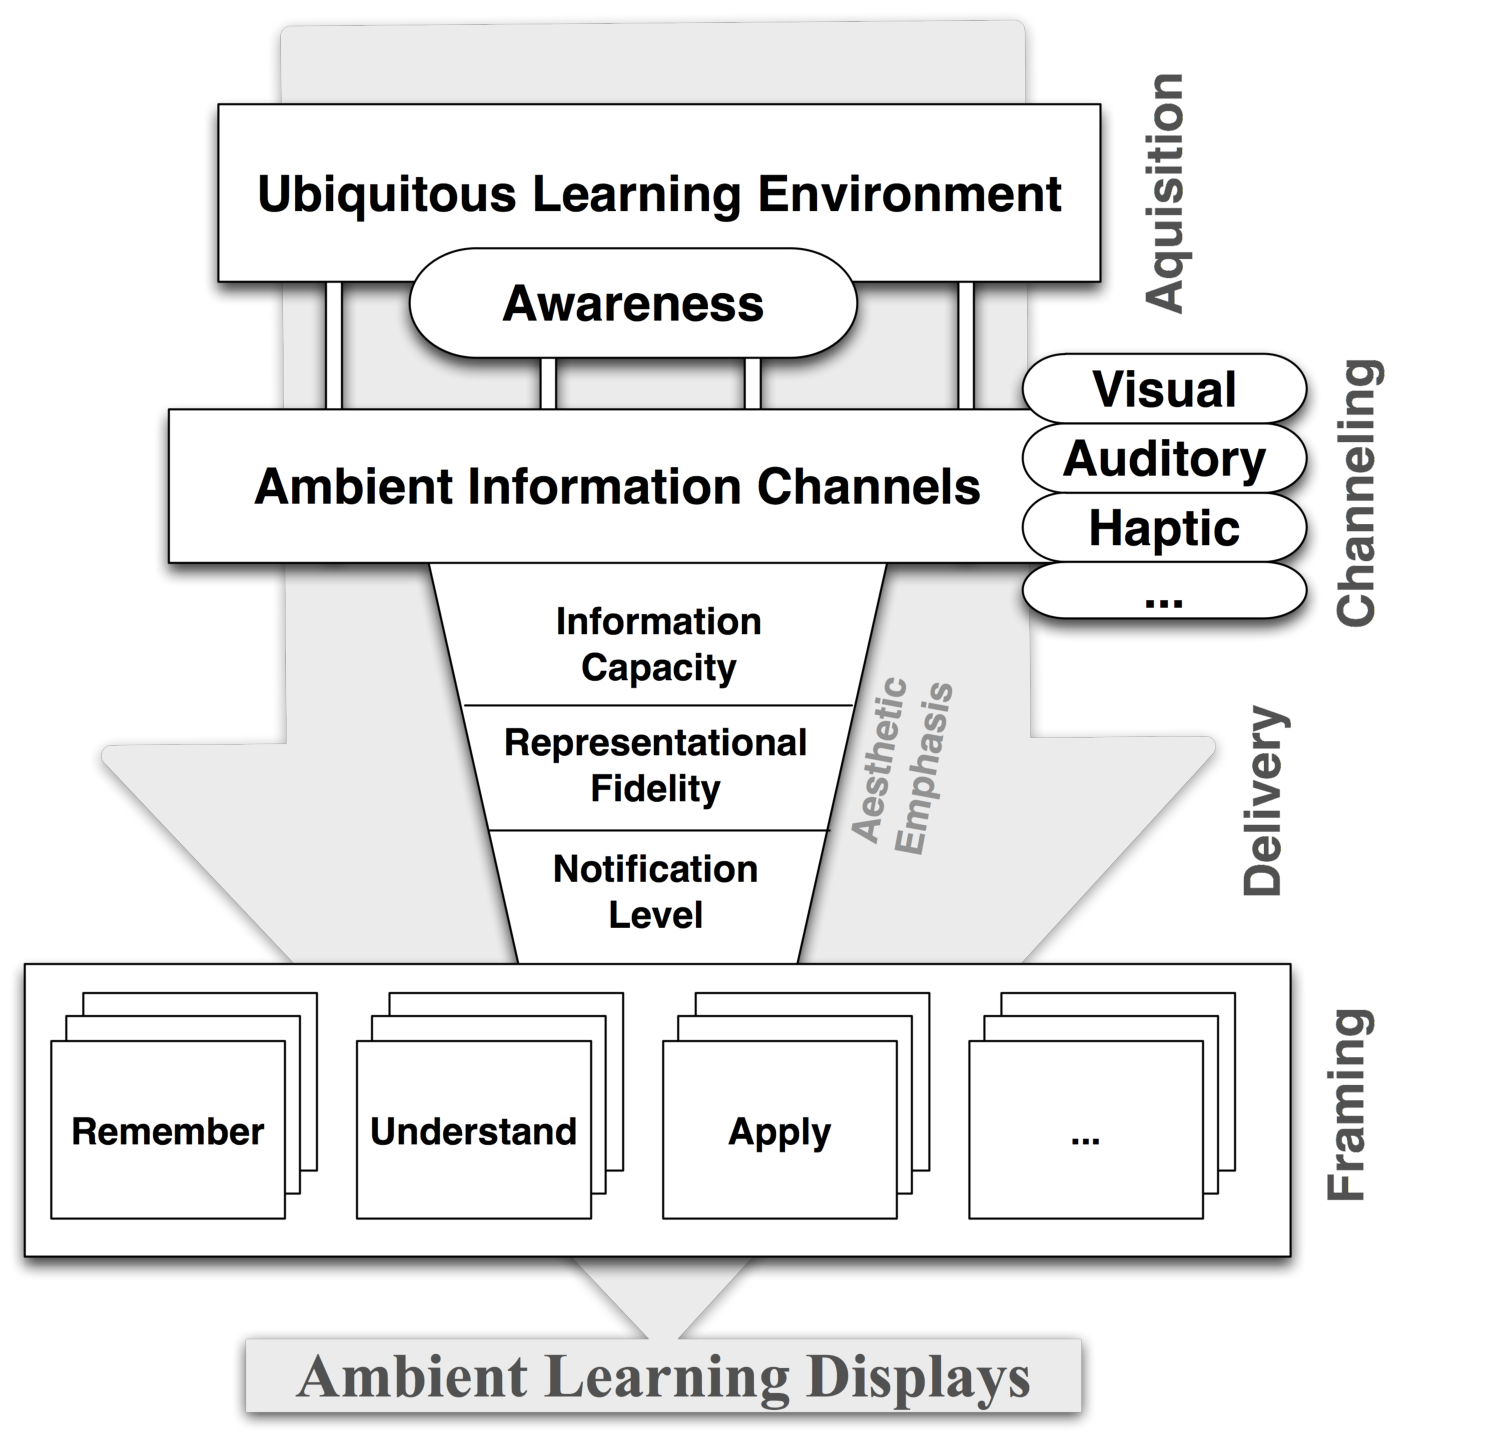
\includegraphics[width=0.9\textwidth]{figures/conceptual_framework}
\caption{Provisional conceptual framework for ambient learning displays} \label{fig:conceptual_framework}
\end{figure}

Within the framework awareness as one of the key concepts for informal learning support
\citep{Syvanen2005a} is used as acquisition instrument of the information relevant for
the learner within the ubiquitous learning environment \citep{Ogata2009b}. Consequently, the
acquired social, task, concept, workspace, knowledge, and context awareness information
sets up the conceptual framework. In order to present the acquired information in context
the ambient information channels model introduced by \citet{Specht2009} is utilised to carry
on the conceptual framework. Within the model ambient channels are used to deliver
information and services but also to feed information back into the system. Thereby,
information might be channelled into visual, auditory, haptic, odorous and respectively
tasting extraditable parts. To deliver the previously channelled information within the
ubiquitous learning environment ambient systems are used. Based on the comparison and
discussion of existing ambient information systems by \citet{Pousman2006b}, the
four design dimensions: information capacity, notification level, representational fidelity,
and aesthetic emphasis are used to design ambient systems as means of delivery. The
framing of the previously acquired, channelled, and delivered information in a learning
context then complements the conceptual framework. Based on the revised taxonomy of
educational objectives of \citet{Anderson2001} activities and objectives
enabled by the systems are matched to the types of knowledge and the cognition
processes involved. Thereby the taxonomy describes on the one hand several cognitive
process dimensions ranging from remembering over applying to creating and
distinguishes on the other factual, conceptual, procedural, and metacognitive knowledge.

But how would relevant information actually flow through the proposed conceptual
framework? Assuming an example setup where the users are asked to identify existing
learning objects/resources available in their proximity and match them according to the
context they are used in. Thereby context describes the relation of a learning scenario and
the location where the scenario takes place. This task addresses a simple cognitive
process dimension dealing with factual knowledge. An ambient system fed with
information reflecting the awareness needs of the users operating within the environment
would be used to support the task. Depending on the activity (derived from the addressed
cognitive process dimension) that needs to be supported, this information is channelled
through ambient information channels utilising different means and modalities to deliver
appropriate input for the ambient systems.

In such a setup creating workspace awareness could mean to use an ambient
visualisation method to describe possible learning scenarios. Concerning knowledge
awareness ambient audification methods could be used to create awareness when
someone enters the environment who created a certain learning object/resource and thus
might assist with the matching. And to provide a last example, vibration could be used as
a possible ambient haptification method to create context awareness reflecting the spatial
proximity of the learning object/resource to its learning scenario, respectively the
designated location.

\section{Research agenda}
Heading towards the implementation and manifestation of the envisioned ambient
learning displays an agenda for further research work has been set up incorporating the
outlined research questions and objectives. Based on this agenda the authors propose a
research project described in the following sections depicting an experimental design as
well as a usable evaluation technique.

In preparation of the research project a small-scale study \citep{Borner2010}\footnote{This publication is included as \textbf{Chapter 4} in this thesis.} has
already been conducted to gather opinion of experts in the field of mobile and ubiquitous
learning on the educational problem that can be solved by mobile learning. For this
purpose Concept Mapping \citep{Trochim1989} has been chosen as an appropriate method.
The method provides a structured approach to identify the experts� opinion on a given
domain, including both qualitative techniques and multivariate analysis approaches. The
result is a visual map of useful and important concepts that can then be used for further
elaborations. The study revealed that the two most important problem clusters are dealing
with �access to learning� and �contextual learning� aspects. Focusing on these problem
clusters and the covered problem descriptions in detail gives valuable insights on the
educational characteristics that define mobile and ubiquitous learning. For the presented
research agenda, these results of the study are used both as indicators for the educational
focus and as an instrument to validate the research findings.

The actual research design will begin with an extensive literature review covering in
general the aspects discussed in Section \ref{sec:ubiquitous_learning_characteristics} with a clear focus on ambient systems.
Regarding ambient systems there is a particular interest in existing applications used to
support personal, social, and environmental sense-making processes; derived patterns for
the design of such applications; and criteria and techniques that have been used for
evaluation. It is expected to find a large number of ambient systems that simply represent
information rather than supporting more complex cognitive processes. In any case, it
needs to be investigated if and how the applications are used within learning scenarios
and how they are evaluated on their effectiveness for learning.

Towards a profound conceptual framework that finally establishes the basis to build
prototypes for an experimental design, a lot of work has already been done as described
in Section \ref{sec:provisional_conceptual_framework}. Under the assumption that the information presented in context needs to
be acquired, channelled, delivered, and framed in the learning process, relevant research
findings, models, design dimensions, and taxonomies have been examined. Though the
outlined provisional conceptual framework for ambient learning systems is still subject of
modifications. Most probably the modifications will be due to the gathered insights from
the literature review of existing ambient systems for learning as well as the evaluation
techniques for respective applications.

\subsection{Experimental design}
Based on the prior literature review and the resulting conceptual framework analysis an
experimental design will be used to evaluate the prototypes built upon the conceptual
framework. Prior to the design it is planned to conduct formative studies to gather
insights on the specific usability needs and requirements of ambient systems and aid the
design process. Then a setup of ambient system prototypes, addressing specific cognitive
process dimensions, varied on the values of single design dimensions will be designed
and implemented. There is a particular interest in the effects on learning affected by the
way the ambient systems present information. The goal is to unveil in summative studies
how the single prototypes and prototype setups perform. The experimental design is
oriented on design-based research \citep{Baumgartner2003}, following a recurrent cycle
of designing an experiment, implementing the experiment, and evaluating the results in
order to review the experimental design again.

An example setup for such an experiment can be illustrated as follows: the ambient
system is fed with information reflecting the awareness needs of users operating within
the ubiquitous learning environment. Depending on the activity (derived from the
addressed cognitive process dimension) that needs to be supported, this information is
channelled through ambient information channels to deliver appropriate input for the
ambient systems. Each ambient design dimension can be varied on its distinguished
values. In this first experimental cycle the effect when manipulating these values on each
dimension will be measured, to figure out if and how this influences the performance of
the given activity and thus is effective for learning or not.

A possible hypothesis in such an experiment would be that ambient systems with a
low information capacity, an abstract representational fidelity, and a level of notification
that only makes aware, benefit the cognitive process dimension �remember�. To test this
hypothesis, the single ambient design dimensions would then be varied and compared to
each other. To do so, quantitative and qualitative data using data logs, questionnaires, as
well as a specific evaluation technique described in the next section will be collected.

\subsection{Evaluation technique} \label{sec:evaluation_technique}
To investigate and determine if the envisioned experimental prototypes are suitable to
support learners in authentic learning situations within ubiquitous learning environments
an appropriate evaluation technique is needed. Due to the nature of ubiquitous learning
finding suitable techniques is rather difficult. Users constantly move across contexts,
change environments, and usually are not restricted to act within a closed testbed for
evaluation. Thus, the experienced conditions cannot be controlled completely nor kept
similar. Therefore traditional evaluation techniques, such as pre-test/post-test designs, are
not sufficient. Instead the evaluation has to be done also in situ, taking into account the
current context, environment, and conditions the user is experiencing.
The challenge though is to find an appropriate technique that allows measuring the
effects in authentic learning situations. For ambient systems as well as ubiquitous
learning applications corresponding methods will be explored during the literature
review. One method that is already in the focus of attention is the experience sampling
method. The method has already been applied and examined for ubiquitous computing
applications. Derived from the field of psychology the technique is especially effective
for learning about situations and person-situation interactions and allows to �take place in
situ, involve several participants, take place over time, and collect both qualitative and
quantitative data� \citep{Consolvo2003a}. The technique uses several brief
adoptable questionnaires to let the participants report about their current activity and the
situation they are in. The participants are alerted in situ and asked to respond by filling
out a brief questionnaire. Traditionally used to evaluate aspects like emotion,
performance, or social interaction, the technique seems also sufficient to evaluate
ambient systems for learning.

Coming back to the example given in the previous section the method could be
applied as follows. Each participant is assigned to a specific task, which is to identify and
match existing objects/resources. To complete the task, the participants need to perform
certain actions. In the moment they completed the assigned task an event is triggered that
delivers an adapted questionnaire taking into account the current situation and context the
participant is in. The participants are then asked to indicate, for example which
information supported them to solve the task or which ambient system supported them to
solve the task. Using statistical methods on the surveyed qualitative and quantitative data
finally allows measuring the effectiveness of the ambient information presentation for
learning through the performance of the participants.

\subsection{Discussion}
While elaborating the research project some issues and challenges mainly related to the
undetermined target domain used to conduct the experiments, the evaluation of
ubiquitous scenarios in laboratory settings, as well as the importance of aesthetic design
for the experiments emerged. The issues related to the application domain are rather
complex. Quite reasonably the chosen application domain has a great influence on the
learning conditions. Authentic and situated learning usually occurs when learners are
strongly related to the placement they are active in and at the same time far away from
traditional (mostly formal) learning capabilities they would usually make use of. The
characteristics of the current placement and the requirements of the learners have in fact a
great influence on the assumptions the learners may have, the conditions they may find in
situ, as well as technical constrains of the settings. The chosen domain has an impact on
the conceptual framework and hence on the experimental design and the evaluation and
thus has to be chosen carefully.

The evaluation of ubiquitous scenarios in laboratory settings is self-contradictory.
While ubiquitous computing and the derived ubiquitous learning scenarios are
characterised by the �anywhere, anytime� paradigm, laboratory settings per se exclude
these features as they postulate the full control of all confounding variables. Evaluation
techniques need to take into account the current context, environment, and conditions the
user is experiencing within the situation that is observed. One possible solution has
already been mentioned in Section \ref{sec:evaluation_technique} describing a method already used to evaluate
ubiquitous computing applications \citep{Consolvo2003a}. Still, other available
methods need to be investigated and verified on their adequacy for the evaluation of
ubiquitous learning applications and thus ambient systems for learning.

Another issue is the importance and influence of an aesthetic design especially when
heading for an end-user product. The aesthetic emphasis is one of the dimensions
affecting the design of ambient systems \citep{Pousman2006b}. Within the
presented research project, this dimension will be mostly ignored. The reason for that is
mainly the focus on evaluating the effects of ambient information presentation on
learning and learning support rather than actually designing end-user products. In this
context emphasising the aesthetics design dimension of ambient systems too much is
simply not feasible for the research project, but definitely needs to be considered when
applying the outcomes to actual learning scenarios.

\section{Conclusions}
The chapter outlines the authors� vision of ambient learning displays � enabling
learners to view, access, and interact with contextualised digital content presented in an
ambient way. The vision is based on a detailed exploration of the characteristics of
ubiquitous learning and a deduction of informational, interactional, and instructional
aspects to focus on. Towards the vision essential research questions and objectives as
well as a conceptual framework that acquires, channels, and delivers the information
framed in the learning process are presented. Furthermore, a research agenda proposing a
research project is presented. This research project offers rich opportunities for the design
of environments following the mobile and ubiquitous learning paradigm, which gain in
importance for technology enhanced learning (TEL). Recently, the EU-funded project
STELLAR identified the grand research challenges for the future of TEL. As a guideline,
three themes have been formulated: connecting learners, orchestrating learning, as well
as contextualising virtual learning environments and instrumentalising learning contexts
\citep{STELLAR2009}. The authors� vision of ambient learning displays is strongly devoted
to the contextualisation theme; implicating manifold overlaps with the other themes.
Therefore the main research outcomes will also flow back into the contextualisation
theme. The main idea behind the theme is to encourage situated learning, while
supporting the learner�s mobility. Building on that, the key research questions in this
theme are:

\begin{compactitem}
  \item How can new forms of contextualised learning enable novel experiences for learners and for development of human competences?  
  \item How to support the mobility of the learner in distributed and multi environment learning settings, like the transition between real and virtual contexts?
  \item Which standards are needed to achieve interoperability and reusability of learning resources in this field? How to harmonise the existing learning standards?
\end{compactitem}

Comparing these key research questions with the presented vision, clarifies the relevance
within the field. The authors� vision of ambient learning displays highlights the
challenges and explores the possibilities that lie in the convergence of mobile and
ubiquitous learning in combination with the utilisation of contextualised digital content
as valuable resources to support learning.

Furthermore, the outlined research project delivers new scientific insights into the
authentic learning support in informal and non-formal learning situations. Within
ubiquitous learning environments the project will investigate if there is a measurable
benefit utilising ambient information presentation for a contextualised learning support.
From a practical point of view this research will flow into a framework that gives
guidelines for the future design of ambient systems for learning.